\section{Introduction}
\begin{frame}{}
  \LARGE RNNs : \textbf{Introduction}
\end{frame}

\begin{frame}{Traditional Language Models}
  \begin{figure}
    \centering
    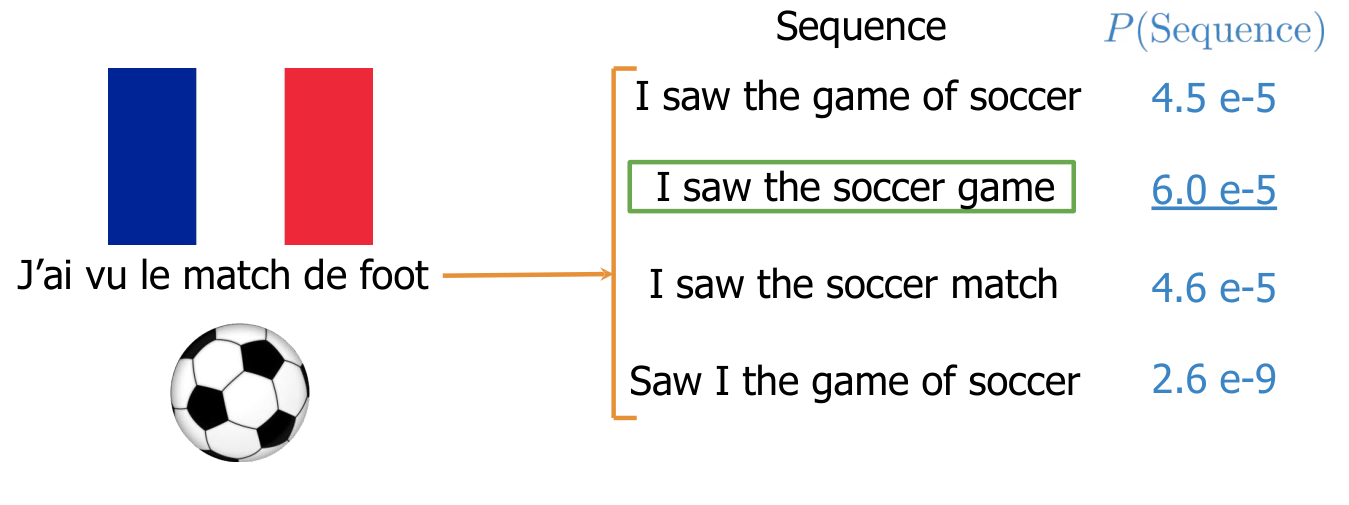
\includegraphics[width=\linewidth,height=0.66\paperheight,keepaspectratio]{images/rnn-lstm-gru/rnn_translation_sequence_probability.png}
    \caption*{\tiny Source: DeepLearning.AI NLP Specialization, Course 3: Natural Language Processing with Sequence Models, Week 2 (Y. Bensouda Mourri \& L. Kaiser)}
  \end{figure}
\end{frame}

\begin{frame}{N-grams}
  \begin{itemize}
      \item Bigrams: $P(w_{2}|w_{1})=\frac{\mathrm{count}(w_{1},w_{2})}{\mathrm{count}(w_{1})}$
      \item Trigrams: $P(w_{3}|w_{1},w_{2})=\frac{\mathrm{count}(w_{1},w_{2},w_{3})}{\mathrm{count}(w_{1},w_{2})}$
      \item $P(w_{1},w_{2},w_{3})=P(w_{1})\times P(w_{2}|w_{1})\times P(w_{3}|w_{1},w_{2})$
      \item \textbf{Limitations:} Large N-grams need significant space and RAM.
  \end{itemize}
\end{frame}

\begin{frame}{N-grams: Limitations}
  \begin{itemize}
      \item N-gram tables consume a lot of memory.
      \item \textbf{Fixed context window:} only the previous $(n-1)$ words are conditioned on.
      \item \textbf{Data sparsity:} larger $n$ implies exponentially many $n$-grams; many combinations are rare or unseen in training data.
      \item \textbf{No learning or adaptability:} probabilities come from counting and normalizing, so nothing is shared between words with similar meanings.
      \item Different types of \textbf{RNNs} are the \textbf{preferred alternative}.
  \end{itemize}
\end{frame}

\begin{frame}{What is an RNN?}
  A neural network with loops allowing information to persist.
  \textbf{Core Elements:}
  \begin{itemize}
      \item Hidden State $h_{t}$ captures memory of previous inputs.
      \item Input $x_{t}$, Output $y_{t}$.
      \item Parameter sharing: Same weights used across time steps.
  \end{itemize}
  \textbf{Mathematical Formulation:}
  \begin{itemize}
      \item $h_{t}=\tanh(W_{hh}h_{t-1}+W_{xh}x_{t}+b_{h})$
      \item $y_{t}=W_{hy}h_{t}+b_{y}$
  \end{itemize}
  \textbf{This recurrence allows information to propagate through time.}
\end{frame}

\begin{frame}{Why Use RNNs?}
  \begin{itemize}
      \item RNNs target \textbf{sequential data} where order matters (language, time series, speech).
      \item \textbf{Capturing context:} a hidden state carries information from previous steps.
      \item Example: word meaning often depends on preceding words; RNNs model such dependency.
      \item \textbf{Variable-length inputs} within a single architecture.
      \item \textbf{Temporal patterns} in language modeling, speech, financial series, etc.
  \end{itemize}
\end{frame}

\begin{frame}{Why Use RNNs?}
  \begin{figure}
    \centering
    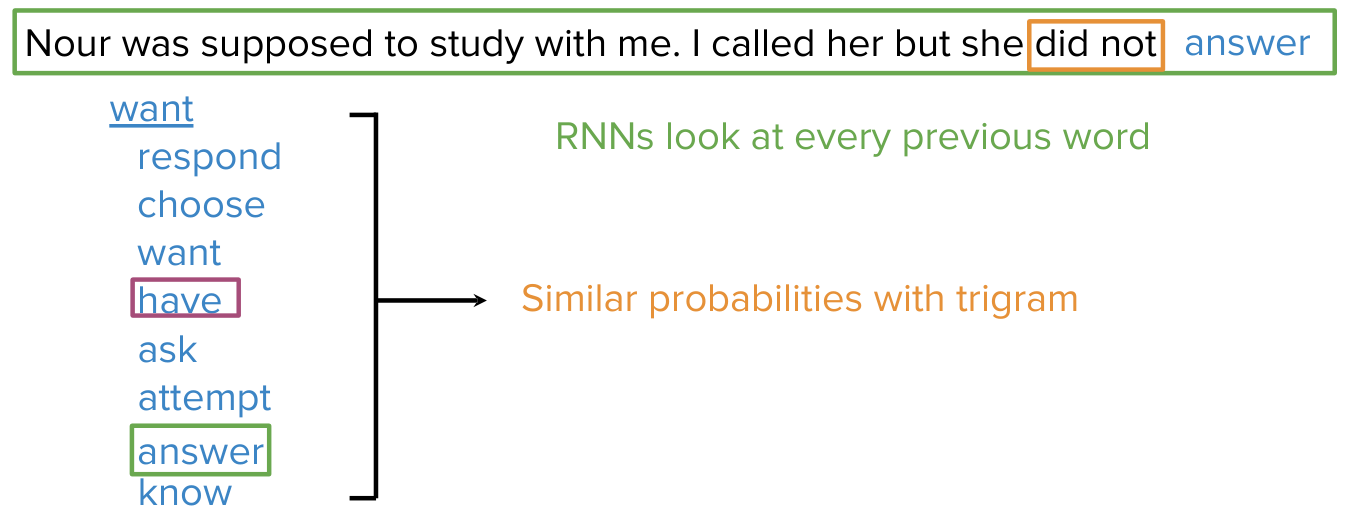
\includegraphics[width=\linewidth,height=0.66\paperheight,keepaspectratio]{images/rnn-lstm-gru/rnn_next_word_prediction_candidates.png}
    \caption*{\tiny Source: DeepLearning.AI NLP Specialization, Course 3: Natural Language Processing with Sequence Models, Week 2 (Y. Bensouda Mourri \& L. Kaiser)}
  \end{figure}
\end{frame}

\begin{frame}{RNNs Basic Structure}
  \begin{figure}
    \centering
    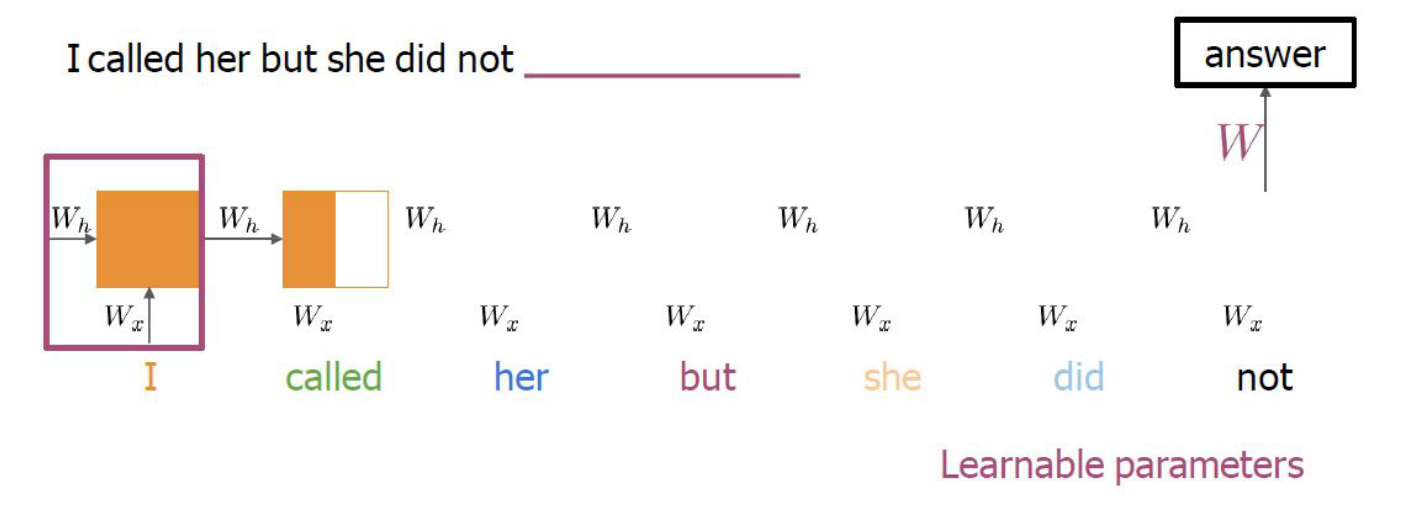
\includegraphics[width=\linewidth,height=0.66\paperheight,keepaspectratio]{images/rnn-lstm-gru/rnn_language_model_next_word.png}
    \caption*{\tiny Source: DeepLearning.AI NLP Specialization, Course 3: Natural Language Processing with Sequence Models, Week 2 (Y. Bensouda Mourri \& L. Kaiser)}
  \end{figure}
\end{frame}
